\section{Déploiement}

Pendant le développement des différents Générateurs de Code, nous avons pu utiliser les outils proposés par Eclipse afin de configurer statiquement le répertoire cible des fichiers à générer lors de l'exécution desdits générateurs. Cette méthodologie nous a permis de définir un Projet \kwplay dédié comme cible de la génération, afin d'effectuer des tests rapidement, sans qu'il ne soit requis de reconfigurer la génération après chaque modification. Le système en place nous a donc permis de tester chaque générateur (pour Entity, SOA, et Cinematic) indépendament.
\\\\
Il n'était cependant pas concevable d'utiliser la même méthodologie pour une \guim{mise en production} du générateur \kwplay. En effet, il n'est pas concevable d'obliger un utilisateur à configurer et lancer manuellement chaque \guim{sous-générateur}, car ceux-ci sont complémentaires (à l'exception peut-être de la génération des WebServices). De plus, il faut dispenser l'utilisateur d'une configuration fastidieuse, et trouver un système plus ergonomique pour que ce dernier puisse lancer rapidement une génération de code.

\subsection{Regroupement des différents générateurs de code}

\subsection{Interface Utilisateur}


\begin{figure}[htb]
  \centering
  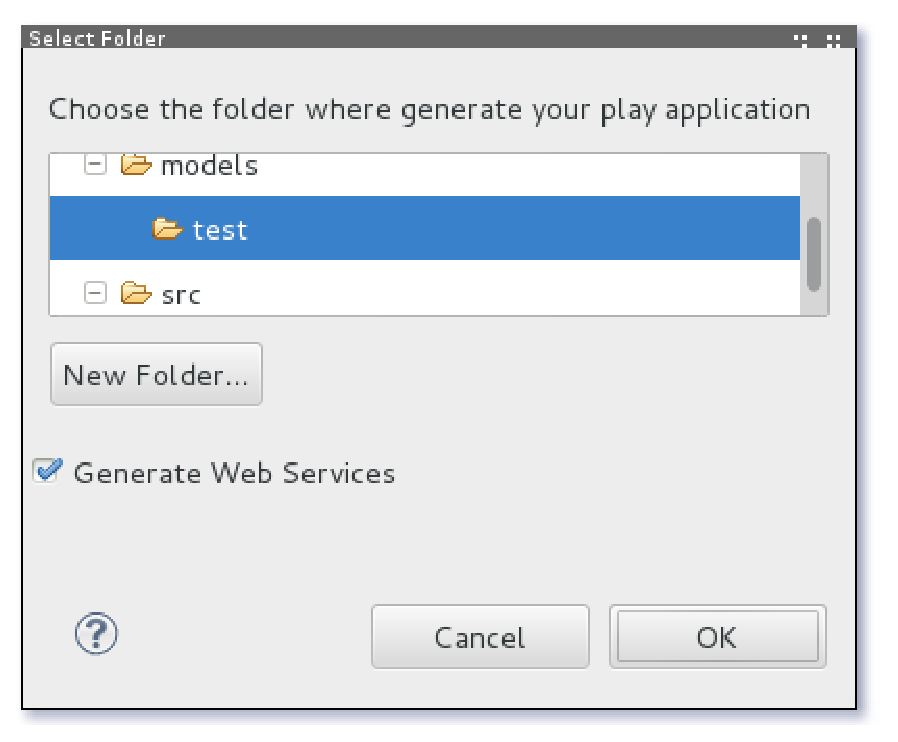
\includegraphics[scale=0.6]{img/screen_ui.eps}
  \caption{Interface Utilisateur pour le lancement du générateur}
  \label{fig:acceleo}
\end{figure}